\thispagestyle{toancuabinone}
\pagestyle{toancuabi}
\everymath{\color{toancuabi}}
\blfootnote{$^1$\color{toancuabi}Trường Liên cấp Hội nhập Quốc tế iSchool Quảng Trị.}
\graphicspath{{../toancuabi/pic2/}}
\begingroup
\AddToShipoutPicture*{\put(0,616){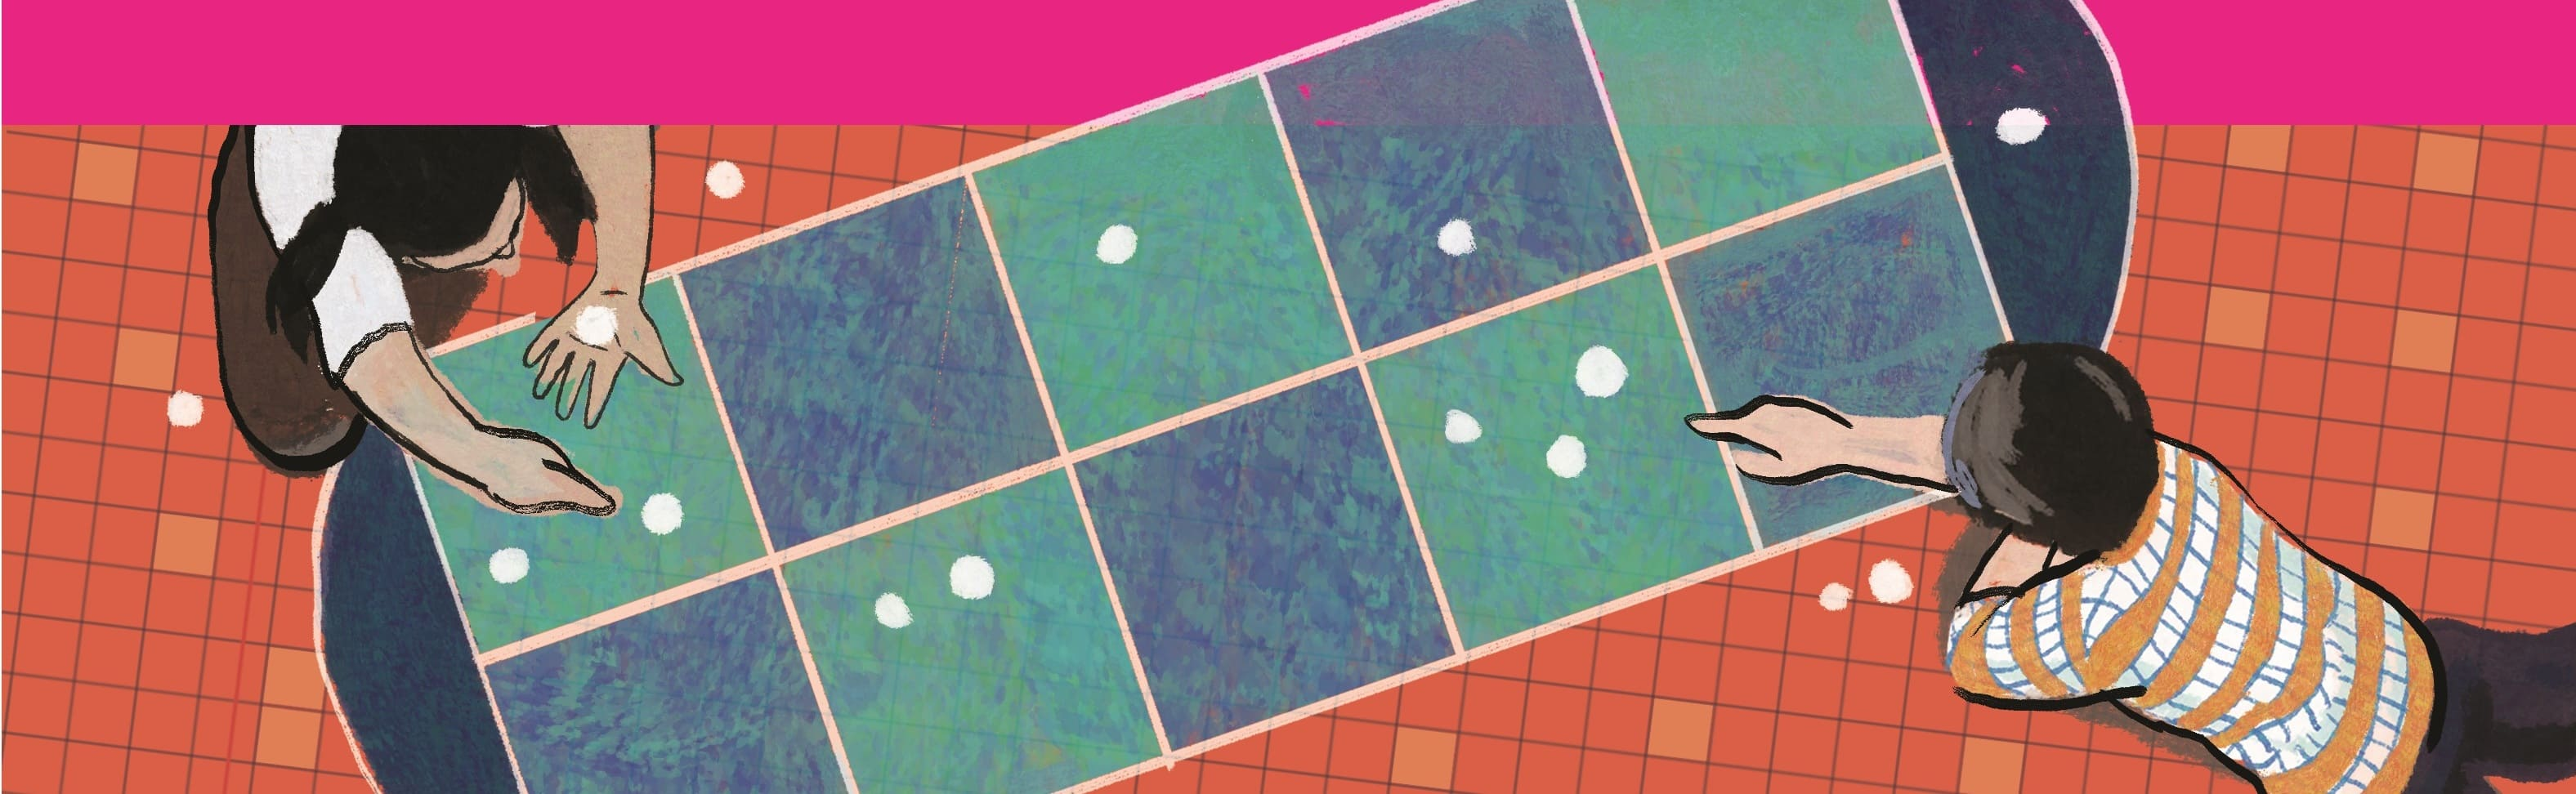
\includegraphics[width=19.3cm]{../bannertoancuabi}}}  
\AddToShipoutPicture*{\put(110,525){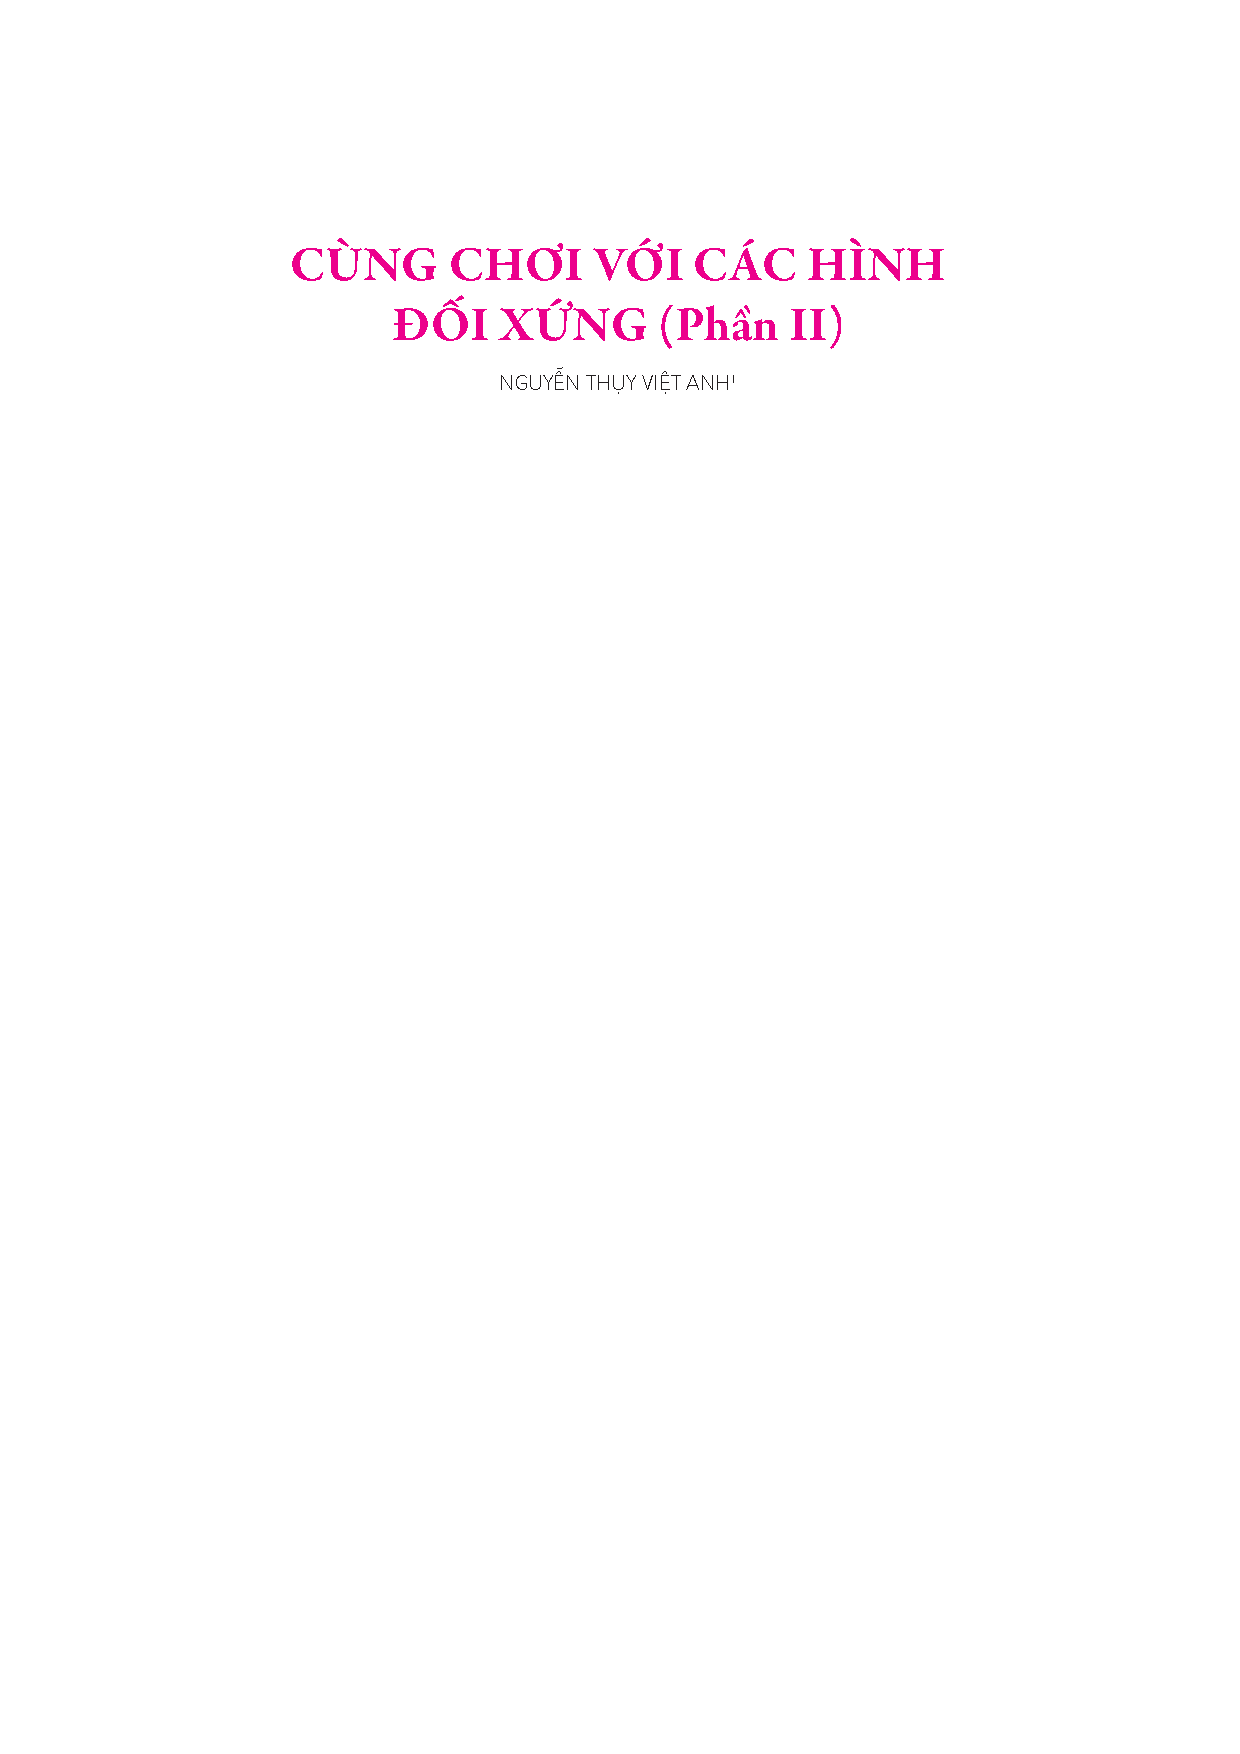
\includegraphics[scale=1]{../tieude10.pdf}}}  
\centering
\endgroup
\vspace*{185pt} 

\begin{multicols}{2}
	Chuồn chuồn tre là sản phẩm độc đáo được các nghệ nhân làng Thạch Xá tạo nên, là món đồ chơi tuổi thơ rất đỗi thân thuộc đối với mỗi người dân trong làng. Lịch sử làng chuồn chuồn tre Thạch Xá với nhiều năm trong nghề đã biến mảnh đất này thành một trong những làng nghề nổi tiếng ở Hà Nội được nhiều du khách biết đến.
	\begin{center}
		\textit{Chuồn chuồn có cánh thì bay\\
			Có thằng cu Tí thò tay bắt chuồn}
	\end{center}
	\hfill \textit{(Đồng dao, thơ ca dân gian)}
	\begin{figure}[H]
		\vspace*{-5pt}
		\centering
		\captionsetup{labelformat= empty, justification=centering}
		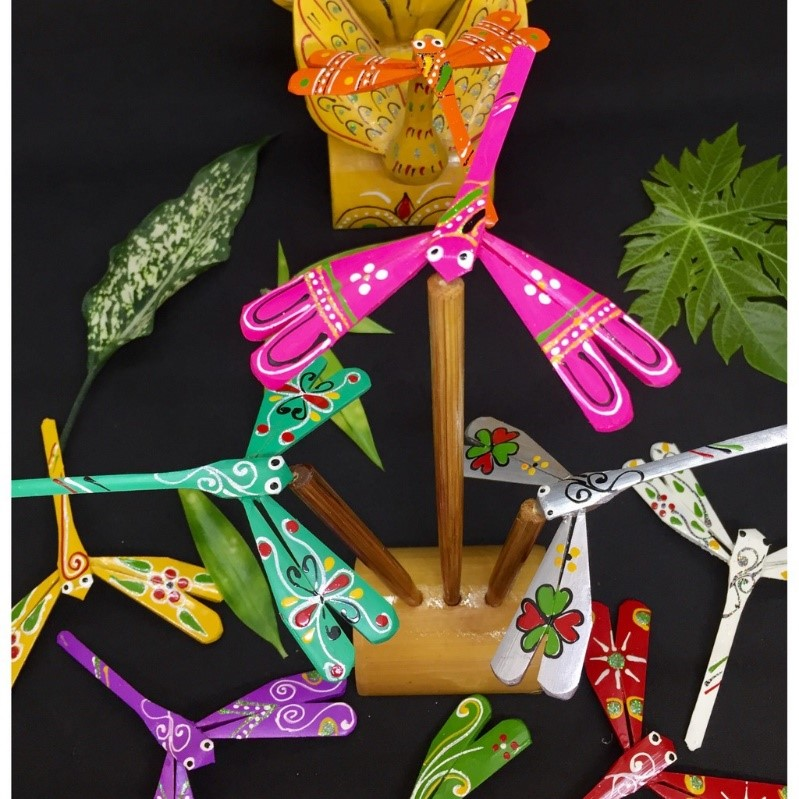
\includegraphics[width= 0.85\linewidth]{10}
		\caption{\small\textit{\color{toancuabi}Ảnh : Internet.}}
		\vspace*{-10pt}
	\end{figure}
	Ngày hôm nay chúng ta sẽ cùng nhau thử sức làm chuồn chuồn tre nhé! Để đơn giản hơn thì chúng ta sẽ thay thế vật liệu để làm chuồn chuồn tre là từ những cây tre thành que kem hoặc giấy.
	\vskip 0.1cm
	\textbf{\color{toancuabi}Cách $\pmb{1}$: Chuồn chuồn que kem thăng bằng}
	\vskip 0.1cm
	\textit{Chuẩn bị nguyên liệu}: 
	\vskip 0.05cm
	-- Các que kem.
	\vskip 0.05cm
	-- Keo, súng bắn keo.
	\vskip 0.05cm
	-- Đũa dùng một lần.
	\vskip 0.05cm
	-- Thước thẳng.
	\vskip 0.05cm
	-- Dao rọc giấy.
	\vskip 0.05cm
	-- Bút chì.
	\vskip 0.05cm
	\textit{Cách làm chuồn chuồn que kem thăng bằng}:
	\vskip 0.1cm
	\textit{Bước} $1$: Sử dụng súng bắn keo dính hai que kem dài $4$ cm lại với nhau.
	\begin{figure}[H]
		\vspace*{-5pt}
		\centering
		\captionsetup{labelformat= empty, justification=centering}
		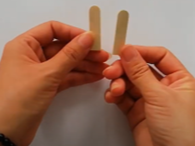
\includegraphics[height=0.37\linewidth]{11}
		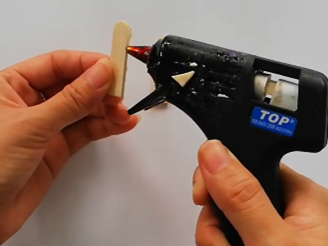
\includegraphics[height=0.37\linewidth]{12}
		
		\vspace*{1pt}
		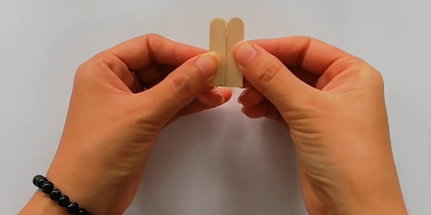
\includegraphics[width=1\linewidth]{13}
%		\vspace*{-5pt}
	\end{figure}
	\textit{Bước} $2$: Sử dụng đầu que kem và bút chì để tạo hình phần đầu cho con chuồn chuồn.
	\begin{figure}[H]
		\vspace*{-5pt}
		\centering
		\captionsetup{labelformat= empty, justification=centering}
		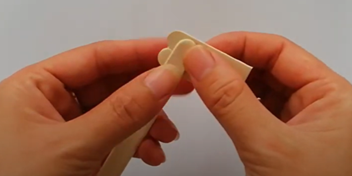
\includegraphics[width=0.7\linewidth]{14}
		
		\vspace*{1pt}
		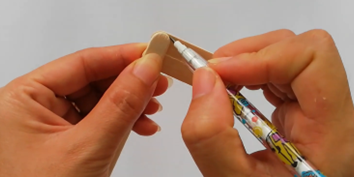
\includegraphics[width=0.7\linewidth]{15}
		
		\vspace*{1pt}
		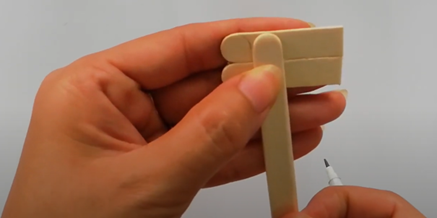
\includegraphics[width=0.7\linewidth]{16}
		
		\vspace*{1pt}
		\hspace*{1pt}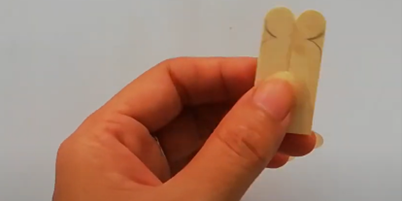
\includegraphics[width=0.7\linewidth]{17}
		\vspace*{-5pt}
	\end{figure}
	\textit{Bước} $3$: Sử dụng dao rọc giấy cắt đi phần khuyết.
	\begin{figure}[H]
		\vspace*{-5pt}
		\centering
		\captionsetup{labelformat= empty, justification=centering}
		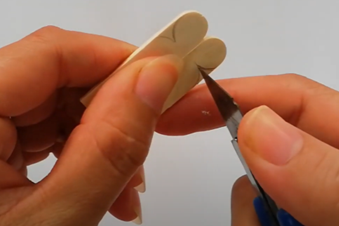
\includegraphics[width=0.7\linewidth]{18}
		
		\vspace*{1pt}
		\hspace*{1pt}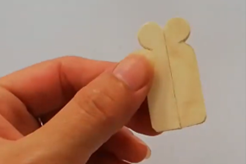
\includegraphics[width=0.7\linewidth]{19}
		\vspace*{-10pt}
	\end{figure}
	\textit{Bước} $4$: Lấy que kem nguyên vẹn rồi cắt chéo đi một nửa (như hình minh họa), sau đó dùng súng bắn keo dán vào que kem dài 10cm để làm cánh chuồn chuồn. (Lưu ý là chuồn chuồn có cánh dài, cánh ngắn).
	\begin{figure}[H]
		\vspace*{5pt}
		\centering
		\captionsetup{labelformat= empty, justification=centering}
		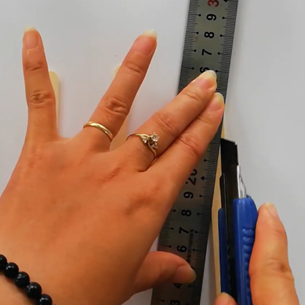
\includegraphics[height=0.35\linewidth]{50}
		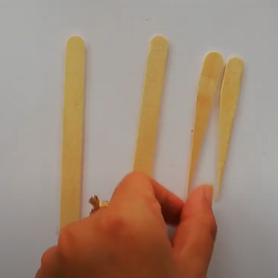
\includegraphics[height=0.35\linewidth]{51}
		
		\vspace*{1pt}
		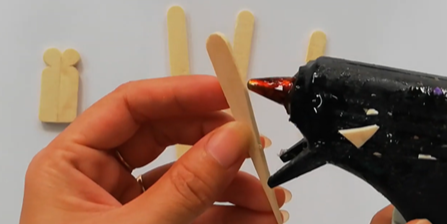
\includegraphics[width=0.7\linewidth]{52}
		
		\vspace*{1pt}
		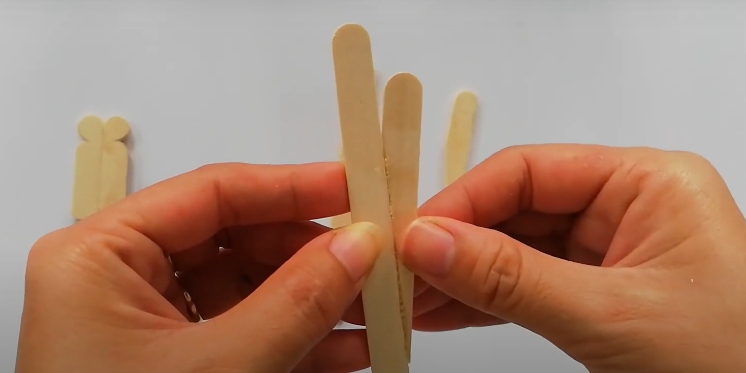
\includegraphics[width=0.7\linewidth]{53}
		
		\vspace*{1pt}
		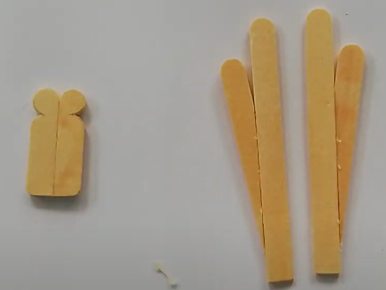
\includegraphics[width=0.7\linewidth]{54}
		\vspace*{-10pt}
	\end{figure}
	\textit{Bước} $5$: Sử dụng súng bắn keo để dán que kem dài $10$ cm vào phần đầu của con chuồn chuồn.
	\begin{figure}[H]
		\vspace*{-5pt}
		\centering
		\captionsetup{labelformat= empty, justification=centering}
		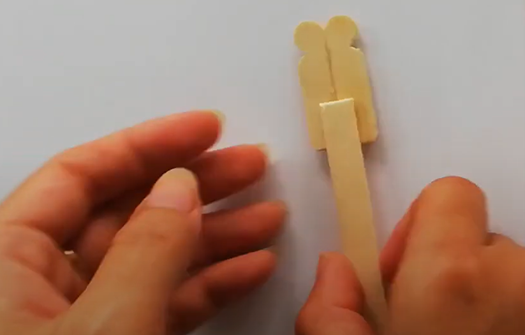
\includegraphics[width=0.7\linewidth]{55}
		\vspace*{-10pt}
	\end{figure}
	\textit{Bước} $6$: Tiếp tục sử dụng súng bắn keo dán hai cánh chuồn chuồn vào thân.
	\begin{figure}[H]
		\vspace*{-5pt}
		\centering
		\captionsetup{labelformat= empty, justification=centering}
		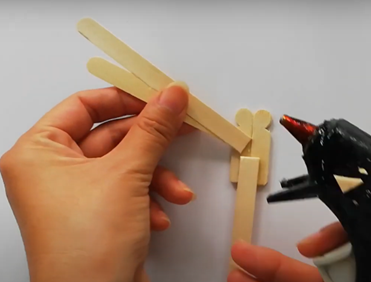
\includegraphics[height=0.36\linewidth]{56}
		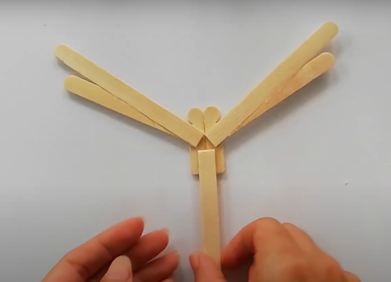
\includegraphics[height=0.36\linewidth]{57}
		\vspace*{-10pt}
	\end{figure}
	\textit{Bước} $7$: Sử dụng súng bắn keo để dán que tre tròn (hoặc đũa dùng một lần) vào chính giữa que kem nguyên vẹn để làm giá đỡ chuồn chuồn.
	\begin{figure}[H]
		\vspace*{5pt}
		\centering
		\captionsetup{labelformat= empty, justification=centering}
		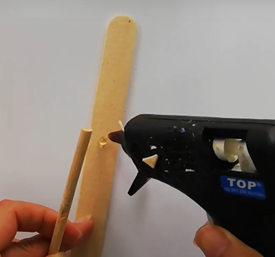
\includegraphics[height=0.34\linewidth]{58}
		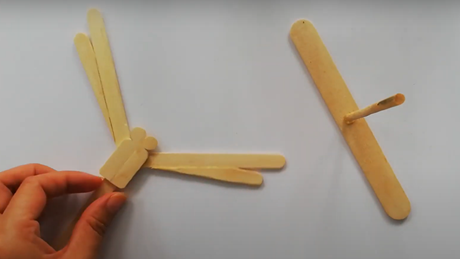
\includegraphics[height=0.34\linewidth]{59}
		\vspace*{-10pt}
	\end{figure}
	Cuối cùng, các em chỉ cần đặt chuồn chuồn lên giá đỡ hoặc lên ngón tay của mình là chuồn chuồn có thể tự thăng bằng được rồi.
	\begin{figure}[H]
		\vspace*{-5pt}
		\centering
		\captionsetup{labelformat= empty, justification=centering}
		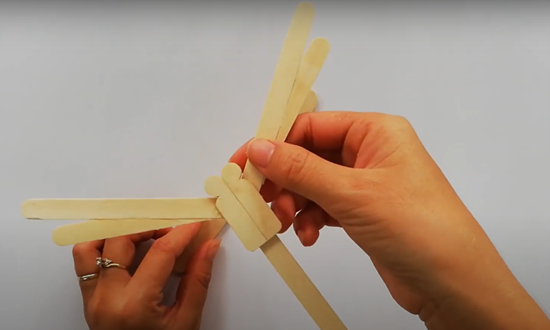
\includegraphics[height=0.35\linewidth]{60}
		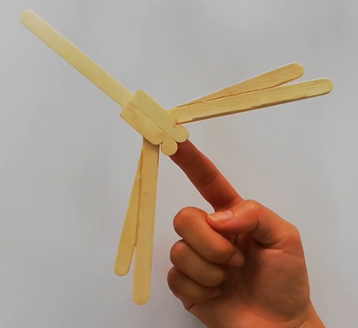
\includegraphics[height=0.35\linewidth]{61}
		\vspace*{-10pt}
	\end{figure}
	\textbf{\color{toancuabi}Cách $\pmb{2}$: Chuồn chuồn giấy thăng bằng}
	\vskip 0.1cm
	\textit{Chuẩn bị nguyên liệu}:
	\vskip 0.1cm
	-- Giấy bìa màu.
	\vskip 0.1cm
	-- Nắp nhựa (tái sử dụng từ chai nhựa bỏ đi).
	\vskip 0.1cm
	-- Đũa dùng một lần.
	\vskip 0.1cm
	-- Bút chì.
	\vskip 0.1cm
	-- Kéo.
	\vskip 0.1cm
	-- Hồ dán.
	\vskip 0.1cm
	-- Keo, súng bắn keo.
	\vskip 0.1cm
	\textit{Cách làm chuồn chuồn giấy thăng bằng}:
	\vskip 0.1cm
	\textit{Bước} $1$: Gấp đôi giấy bìa màu hình chữ nhật (có chiều dài $13$ cm và chiều rộng $4$ cm).
	\begin{figure}[H]
		\vspace*{-5pt}
		\centering
		\captionsetup{labelformat= empty, justification=centering}
		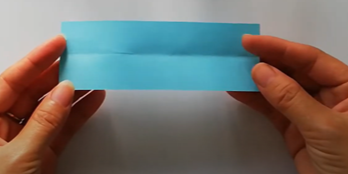
\includegraphics[width=0.7\linewidth]{62}
		
		\vspace*{1pt}
		\hspace*{1pt}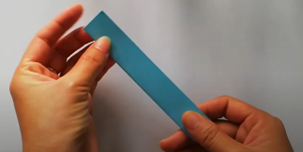
\includegraphics[width=0.7\linewidth]{63}
		\vspace*{-10pt}
	\end{figure}
	\textit{Bước} $2$: Sử dụng bút chì vẽ hình dạng con chuồn chuồn lên tờ giấy màu, sau đó dùng kéo cắt ra.
	\begin{figure}[H]
		\vspace*{5pt}
		\centering
		\captionsetup{labelformat= empty, justification=centering}
		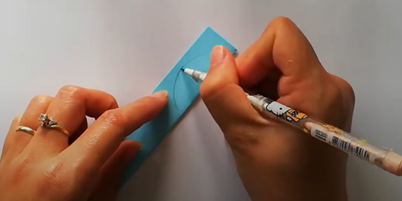
\includegraphics[width=0.7\linewidth]{64}
		
		\vspace*{1pt}
		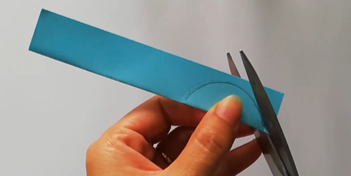
\includegraphics[width=0.7\linewidth]{65}
		
		\vspace*{1pt}
		\hspace*{1pt}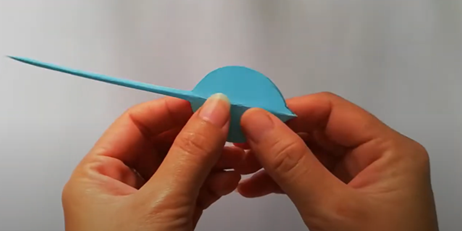
\includegraphics[width=0.7\linewidth]{66}
		\vspace*{-10pt}
	\end{figure}
	\textit{Bước} $3$: Gấp đôi giấy bìa màu hình chữ nhật (có chiều dài $11$ cm và chiều rộng $5$ cm).
	\begin{figure}[H]
		\vspace*{-5pt}
		\centering
		\captionsetup{labelformat= empty, justification=centering}
		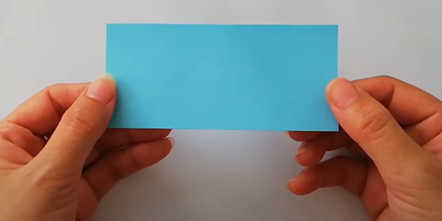
\includegraphics[width=0.7\linewidth]{67}
		
		\vspace*{1pt}
		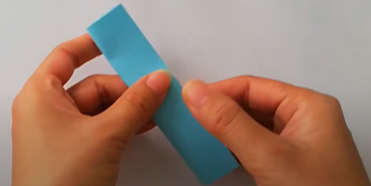
\includegraphics[width=0.7\linewidth]{68}
		\vspace*{-10pt}
	\end{figure}
	\textit{Bước} $4$: Sử dụng bút chì vẽ hình dạng cánh chuồn chuồn lên tờ giấy màu, sau đó dùng kéo cắt ra.
	\begin{figure}[H]
		\vspace*{-5pt}
		\centering
		\captionsetup{labelformat= empty, justification=centering}
		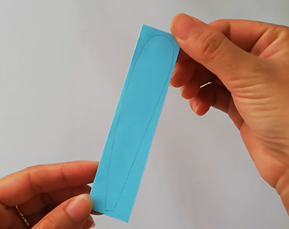
\includegraphics[height=0.31\linewidth]{69}
		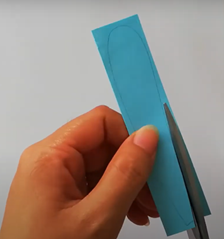
\includegraphics[height=0.31\linewidth]{70}
		
		\vspace*{1pt}
		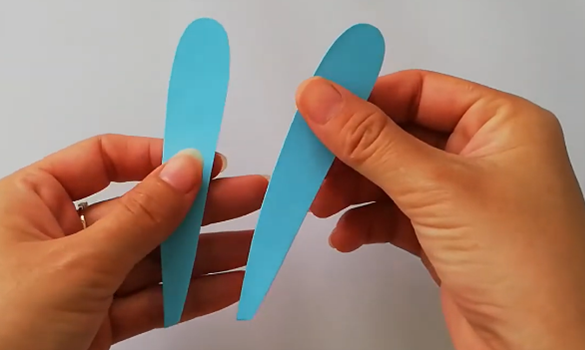
\includegraphics[width=0.7\linewidth]{71}
		\vspace*{-10pt}
	\end{figure}
	\textit{Bước} $5$: Làm tương tự với giấy bìa màu hình chữ nhật (có chiều dài $9$ cm và chiều rộng $4{,}5$~cm) để tạo ra hai cánh nhỏ hơn cho chuồn chuồn.
	\begin{figure}[H]
		\vspace*{-5pt}
		\centering
		\captionsetup{labelformat= empty, justification=centering}
		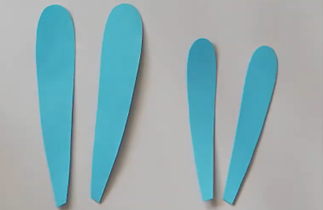
\includegraphics[width=0.7\linewidth]{72}
		\vspace*{-10pt}
	\end{figure}
	\textit{Bước} $6$: Sử dụng hồ dán để dán cánh chuồn chuồn vào thân chuồn chuồn.
	\begin{figure}[H]
		\vspace*{-5pt}
		\centering
		\captionsetup{labelformat= empty, justification=centering}
		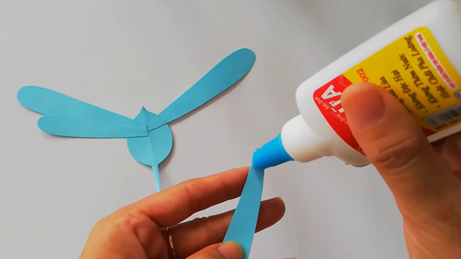
\includegraphics[width=0.7\linewidth]{73}
		\vspace*{-10pt}
	\end{figure}
	\textit{Bước} $7$: Sử dụng súng bắn keo để dán que tre tròn (hoặc đũa dùng một lần) vào chính giữa nắp nhựa để làm giá đỡ chuồn chuồn.
	\begin{figure}[H]
		\vspace*{5pt}
		\centering
		\captionsetup{labelformat= empty, justification=centering}
		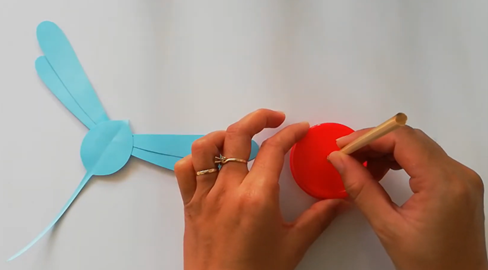
\includegraphics[width=0.7\linewidth]{74}
		\vspace*{-10pt}
	\end{figure}
	Cuối cùng, đặt chuồn chuồn giấy lên giá đỡ hoặc lên ngón tay của mình là chuồn chuồn có thể tự thăng bằng được rồi.
	\begin{figure}[H]
		\vspace*{-5pt}
		\centering
		\captionsetup{labelformat= empty, justification=centering}
		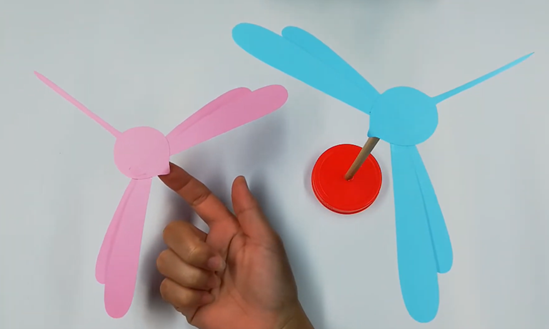
\includegraphics[width=0.7\linewidth]{75}
		\vspace*{-10pt}
	\end{figure}
	\textbf{\color{toancuabi}Tài liệu tham khảo}
	\vskip 0.1cm
	\url{https://www.youtube.com/watch?v=xuiet}\\ \url{oqtOlw}
	\vskip 0.1cm
	\url{https://www.youtube.com/watch?v=uRA}\\ \url{T1t6w2lU}
\end{multicols}
\vspace*{-15pt}
{\color{toancuabi}\rule{1\linewidth}{0.1pt}}
\graphicspath{{../toancuabi/pic/}}
\begingroup
\AddToShipoutPicture*{\put(54,340){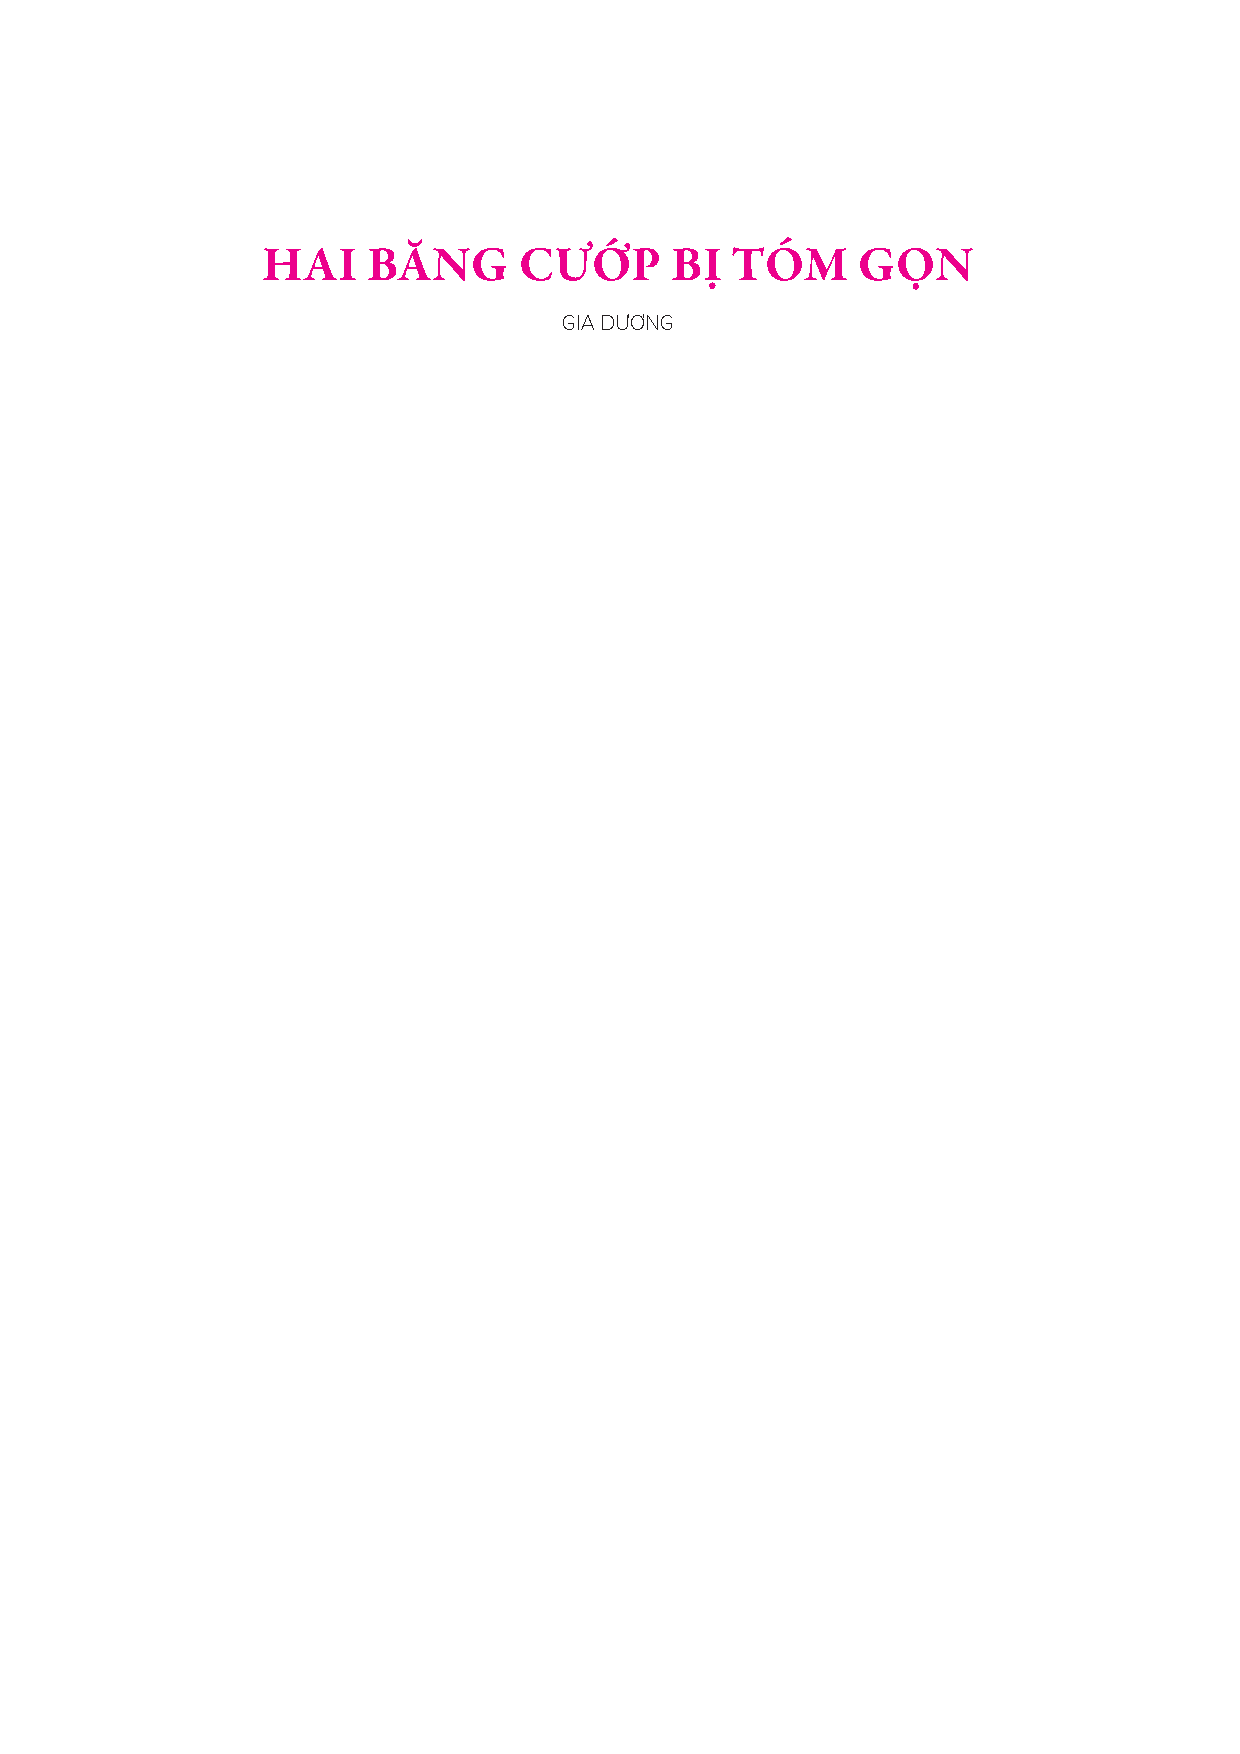
\includegraphics[scale=1]{../tieude.pdf}}}  
\centering
\endgroup
\vspace*{35pt} 
\begin{multicols}{2}
	Thám tử Xuân Phong cần tổ chức một cuộc điều tra tất cả các nhân viên của một công ty vận tải để nắm bắt được tình hình an ninh trật tự của thành phố trong mùa du lịch. Xuân Phong được biết rằng các nhân viên này chia ra thành $3$ loại: những người trung thực, những người nói dối và những người ranh mãnh. Tất cả các nhân viên, do phục vụ gần nhau trong cùng một công ty, nên đều biết nhau và biết ai là thuộc loại người nào. Xuân Phong nhờ cô thư ký xinh đẹp in sẵn những tờ phiếu điều tra để phát cho họ với câu hỏi duy nhất: ``Bạn hãy cho biết trong số các nhân viên của công ty có bao nhiêu người trung thực?". Những người trung thực đã trả lời chính xác, những người nói dối tất nhiên trả lời hoàn toàn sai, còn những người ranh mãnh thì tuỳ ý (có người trả lời đúng và cũng có người trả lời sai). Tất cả các phiếu sau khi thu về đều ghi một số có hai chữ số. Sau khi cô thư ký tổng hợp kết quả, Xuân Phong nhận thấy chữ số $3$ đã được viết ra $33$ lần, chữ số $5$ được viết ra $66$ lần, còn chữ số $7$ được viết ra $77$ lần. Ngoài ra không có chữ số nào khác được ghi trên các phiếu điều tra được thu về. Các em hãy thử đoán xem có tất cả bao nhiêu nhân viên trung thực làm việc trong công ty đó?
%	Lời giải
%	\vskip 0.1cm
%	Do tất cả các nhân viên trung thực đều viết đúng số lượng, chỉ sử dụng các chữ số $3$, $5$ hoặc $7$, suy ra ta chỉ cần xét $9$ trường hợp đối với số lượng các nhân viên trung thực: 
%	\begin{align*}
%		33,35,37,53,55,57,73,75,77.
%	\end{align*}
%	Chữ số $3$ được viết $33$ lần. Vì thế, số người trung thực không thể là $33$ (vì nếu không những người trung thực sẽ viết ra chữ số $3$ tận $66$ lần). Cũng vậy số người trung thực không thể là $35$, $37$, $53$ hoặc $73$, vì nếu không những người trung thực sẽ viết ra chữ số $3$ nhiều hơn $33$ lần.
%	\vskip 0.1cm
%	Chữ số $5$ được viết ra $66$ lần. Do  đó, số người trung thực không thể là $55$ (vì nếu không họ sẽ viết ra tận $110$ lần chữ số $5$), và cũng không thể là $75$ (vì nếu không, những người trung thực sẽ viết ra $75$ lần chữ số $5$).
%	\vskip 0.1cm
%	Số những người trung thực cũng không thể là $77$, vì nếu không những người trung thực sẽ viết ra $154$ lần chữ số $7$. 
%	\vskip 0.1cm
%	Còn lại duy nhất một khả năng là có $57$ người trung thực. Có rất nhiều trường hợp có thể xảy ra tương ứng với đáp số này, các em không nhất thiết phải tìm ra cụ thể tất cả các trường hợp.
%	\vskip 0.1cm
%	Ví dụ, có $9$ người ranh mãnh cũng viết số $57$, trong số những người còn lại có $11$ người gồm cả những người nói dối và những người ranh mãnh sẽ viết trả lời là số $33$, còn $11$ người (gồm cả những người nói dối và những người ranh mãnh) viết trả lời là số $73$.
	\begin{figure}[H]
		\centering
		\vspace*{-5pt}
		\captionsetup{labelformat= empty, justification=centering}
		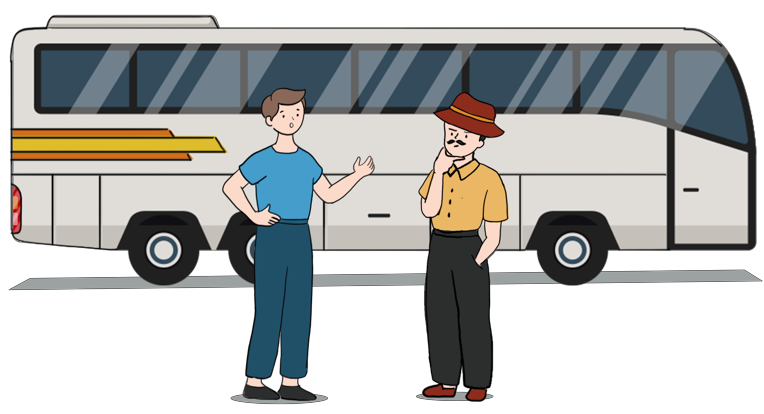
\includegraphics[width=1\linewidth]{xp}
%		\vspace*{5pt}
	\end{figure}
\end{multicols}
\newpage
%\vspace*{-10pt}
%{\color{toancuabi}\rule{1\linewidth}{0.1pt}}
\begingroup
\AddToShipoutPicture*{\put(115,672){
\includegraphics[scale=1]{../tieude11.pdf}}} 
\centering
\endgroup
\vspace*{32pt}

\begin{multicols}{2}
	$\pmb{1.}$ 	Tại thành phố Hoa Hướng Dương, trong số các cậu bé tí hon có $5$ cậu ngày nào cũng ăn bánh rán ngọt, có $7$ cậu bé cứ cách một ngày lại ăn bánh rán ngọt, còn tất cả các cậu bé tí hon còn lại không bao giờ ăn bánh rán ngọt. Ngày hôm qua có $9$ cậu bé tí hon đã ăn bánh rán ngọt. Hỏi trong ngày hôm nay sẽ có bao nhiêu cậu bé tí hon ăn bánh rán ngọt?
	\begin{figure}[H]
		\centering
		\vspace*{-5pt}
		\captionsetup{labelformat= empty, justification=centering}
		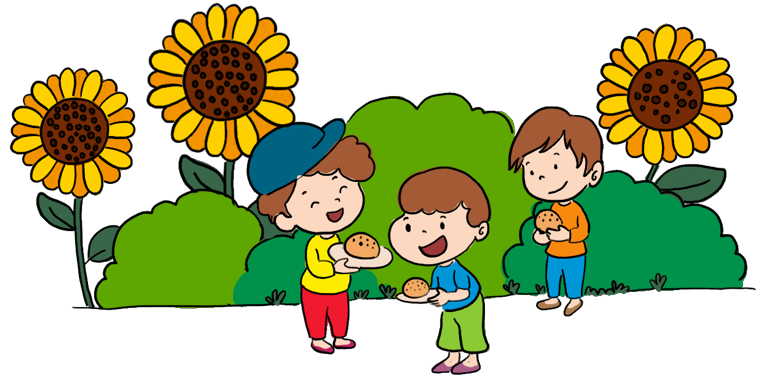
\includegraphics[width=1\linewidth]{Pi9_bai1}
		\vspace*{-15pt}
	\end{figure}
	$\pmb{2.}$ Một cửa hàng bán hoa tươi có ba loại hoa hồng: hồng tím, hồng vàng và hồng đỏ. Số hoa hồng tím bằng một nửa tổng số hoa hồng vàng và hồng đỏ. Số hoa hồng đỏ lại bằng một phần ba tổng số hoa hồng vàng và số hoa hồng tím. Biết rằng số hoa hồng vàng là $45$ bông. Hỏi cửa hàng có bao nhiêu hoa hồng tím và hoa hồng đỏ?
	\begin{figure}[H]
		\centering
		\vspace*{-5pt}
		\captionsetup{labelformat= empty, justification=centering}
		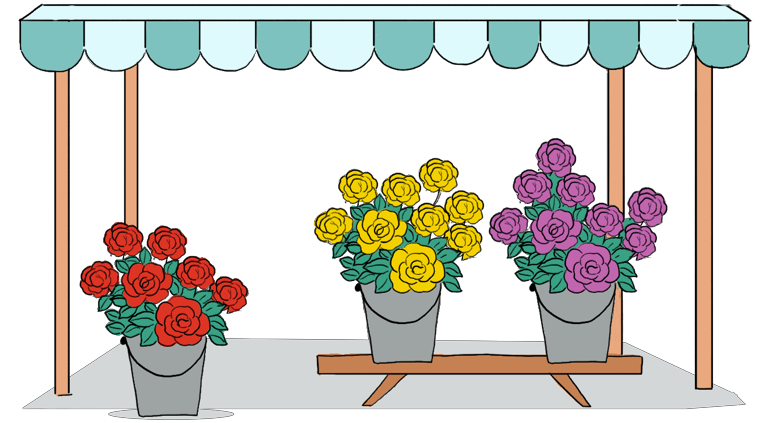
\includegraphics[width=1\linewidth]{Pi9_bai2}
		\vspace*{-15pt}
	\end{figure}
	$\pmb{3.}$ Thỏ Hồng đi đón $3$ cậu bạn của mình là Ngựa Đốm, Ngựa Bạch và Gấu Nâu lặn lội đến thăm nhà mình. Vừa ra tới bìa rừng, Thỏ Hồng đã thấy lờ mờ ba bạn đứng hàng ngang ở xa xa ngoài bãi cỏ, nhưng vì sương mù dày đặc, Thỏ Hồng không thể nhận ra ai với ai. Thỏ Hồng bèn kêu các bạn tự giới thiệu để biết được từng vị khách. Cậu bạn đứng ở ngoài cùng bên trái từ vị trí quan sát của Thỏ Hồng nói rằng: ``Có Gấu Nâu đứng cạnh tôi đấy". Cậu bạn đứng ở ngoài cùng bên tay phải, lại tuyên bố rằng: ``Đó là Ngựa Bạch vừa nói với cậu đấy". Cuối cùng, cậu bạn đứng ở giữa, thông báo rằng: ``Bên tay trái của tôi là Ngựa Đốm đấy". Các em hãy tìm ra bạn nào đứng ở đâu trong số $3$ người bạn của Thỏ Hồng, biết rằng Ngựa Đốm thì chuyên nói dối, Ngựa Bạch thì thỉnh thoảng nói dối, còn Gấu Nâu thì không bao giờ nói dối Thỏ Hồng.
	\begin{figure}[H]
		\centering
		\vspace*{-5pt}
		\captionsetup{labelformat= empty, justification=centering}
		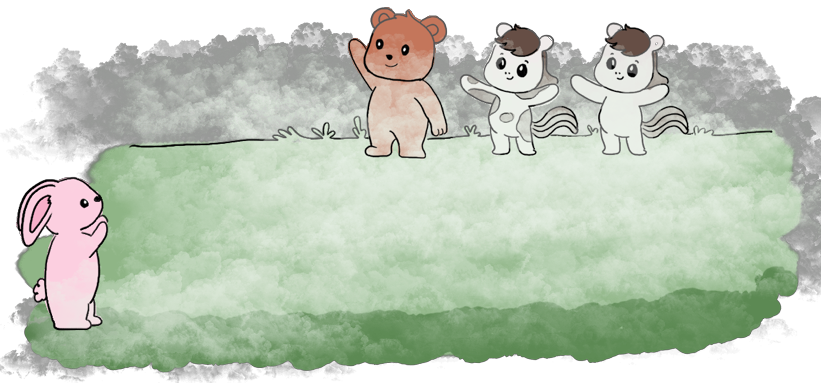
\includegraphics[width=1\linewidth]{Pi9_bai3}
		\vspace*{-15pt}
	\end{figure}
	$\pmb{4.}$ Có $7$ quả táo, khối lượng mỗi quả có thể khác nhau để ở trên bàn. Bạn Thanh nhận thấy rằng có thể đặt $3$ quả trên một đĩa cân và $4$ quả còn lại trên đĩa cân bên kia sao cho hai bên cân thăng bằng. Bạn Thịnh lại thấy rằng có thể đặt $2$ quả táo trên một đĩa cân, và $5$ quả còn lại trên đĩa cân bên kia và hai bên cân cũng thăng bằng. Em hãy chỉ ra rằng có thể đặt trên một đĩa cân bên này $1$ quả táo và đặt trên đĩa cân bên kia $3$ quả táo trong số $7$ quả đã cho, sao cho hai bên cân cũng vẫn thăng bằng.
	\begin{figure}[H]
		\centering
		\vspace*{-5pt}
		\captionsetup{labelformat= empty, justification=centering}
		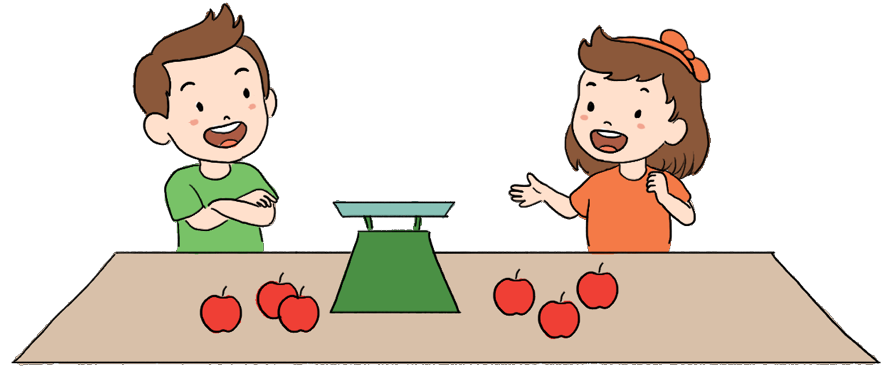
\includegraphics[width=1\linewidth]{Pi9_bai4}
		\vspace*{-15pt}
	\end{figure}
	$\pmb{5.}$ Có $20$ chiếc túi nilon, mỗi túi đựng $26$ quả mận. Biết rằng tổng khối lượng của mỗi túi không vượt quá $1$ kg. Em hãy chỉ ra rằng có thể xếp số mận trên vào $26$ chiếc túi nilon, mỗi túi có đúng $20$ quả mận, sao cho tổng khối lượng của mỗi túi nhỏ hơn $1$ kg.
	\begin{figure}[H]
		\centering
		\vspace*{-5pt}
		\captionsetup{labelformat= empty, justification=centering}
		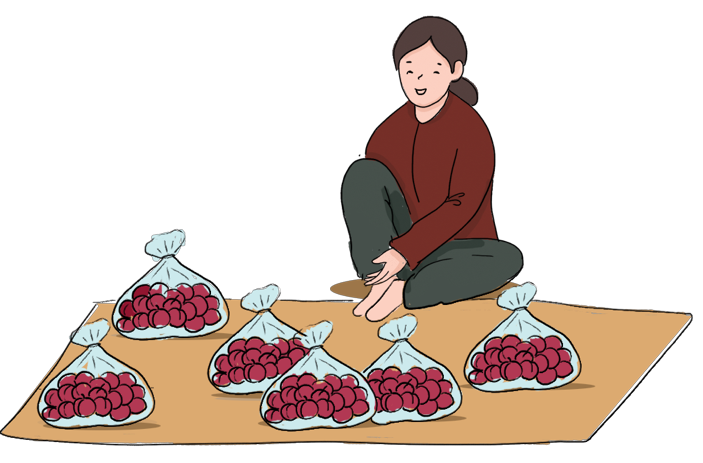
\includegraphics[width=0.8\linewidth]{Pi9_bai5}
		\vspace*{-5pt}
	\end{figure}
	$\pmb{6.}$ 	Có $100$ số $1, 2, 3, \ldots, 100$ được viết ra thành hàng ngang từ trái qua phải theo thứ tự tăng dần. Bạn Long và bạn Lâm chơi một trò chơi như sau. Hai bạn lần lượt đến lượt chơi của mình sẽ đặt duy nhất một trong các dấu $+$, $-$ hoặc $\times$ vào vị trí bất kỳ xen kẽ giữa hai số trong $100$ số nói trên. Bạn đi lượt cuối cùng sẽ thắng nếu số nhận được bằng cách thực hiện phép tính bởi $100$ số và các phép tính đã điền giữa chúng là một số lẻ. Em hãy chỉ ra rằng nếu Long là người đi đầu tiên (và cũng sẽ là người đi cuối cùng) thì Long luôn có cách chơi để thắng.
	\begin{figure}[H]
		\centering
		\vspace*{-5pt}
		\captionsetup{labelformat= empty, justification=centering}
		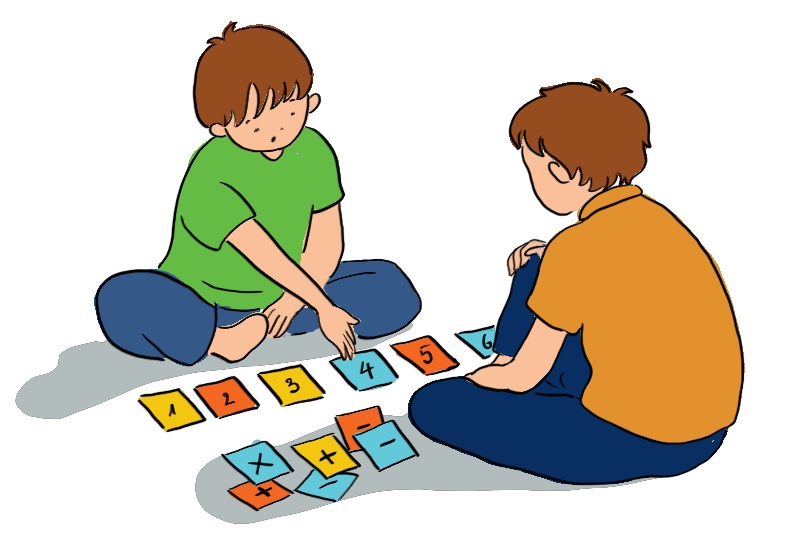
\includegraphics[width=0.7\linewidth]{Pi9_bai6}
		\vspace*{-5pt}
	\end{figure}
\end{multicols}
\vspace*{-10pt}
{\color{toancuabi}\rule{1\linewidth}{0.1pt}}
%\newpage
\begingroup
\AddToShipoutPicture*{\put(112,360){
\includegraphics[scale=1]{../tieude2.pdf}}} 
\centering
\endgroup
\vspace*{75pt}

\begin{multicols}{2}
	$\pmb{1.}$	Trong một cuộc thi thể thao, ban tổ chức chọn ra một số bạn học sinh ở lớp $5A$ và một số bạn ở lớp $5B$ thi đấu trực tiếp. Mỗi bạn ở lớp $5A$ được chọn ra sẽ thi đấu duy nhất một trận với một bạn ở lớp $5B$, và ngược lại, mỗi bạn ở lớp $5B$ được chọn ra chỉ đấu đúng một trận với một bạn ở lớp $5A$.
	\begin{figure}[H]
		\centering
		\vspace*{-5pt}
		\captionsetup{labelformat= empty, justification=centering}
		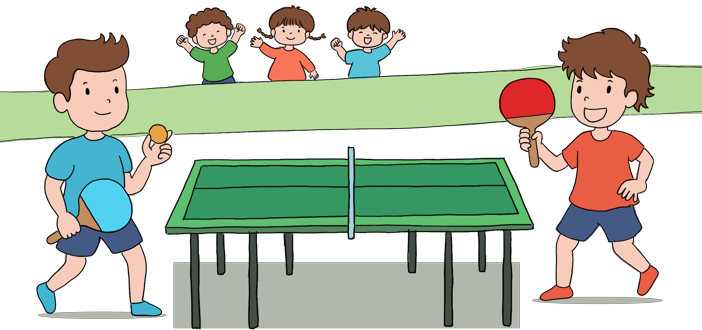
\includegraphics[width=1\linewidth]{Pi5_bai1}
		\vspace*{-10pt}
	\end{figure}
	Biết rằng số học sinh lớp $5A$ được chọn thi đấu chiếm $2/3$ tổng số học sinh toàn lớp $5A$, còn số học sinh lớp $5B$ được chọn thi đấu chiếm $3/5$ tổng số học sinh toàn lớp $5B$. Tổng số học sinh của cả hai lớp là $57$ bạn. Hỏi có bao nhiêu học sinh của hai lớp đã tham gia các trận thi đấu trực tiếp?
	\vskip 0.1cm
	\textit{Lời giải.} 	Gọi số trận thi đấu được tổ chức là $n$. Khi đó số học sinh của lớp $5A$ là $\dfrac{3}{2}\cdot n$, và số học sinh của lớp $5B$ là $\dfrac{5}{3}\cdot n$. Tổng số học sinh của hai lớp sẽ bằng  
	\begin{align*}
		\frac{3}{2}\cdot n + \frac{5}{3}\cdot n = (\frac{3}{2} + \frac{5}{3})\cdot n = \frac{19}{6}n = 57.
	\end{align*}
	Vì vậy $n=18$. 
	\vskip 0.1cm
	Do mỗi trận đấu có hai học sinh tham gia, nên số học sinh của hai lớp đã tham gia các trận thi đấu trực tiếp là $18 \times 2=36$ (học sinh).
	\vskip 0.1cm
	$\pmb{2.}$ Công ty vận tải được thông báo ngắn gọn là có một số kiện hàng có tổng khối lượng là $10$ tấn cần được vận chuyển, hơn nữa mỗi kiện hàng nặng không quá $1$ tấn. Hỏi công ty  cần điều động ít nhất bao nhiêu xe tải có trọng tải là $3$ tấn mỗi xe để luôn chắc chắn chở được hết được số hàng hoá đó?
	\begin{figure}[H]
		\centering
		\vspace*{-5pt}
		\captionsetup{labelformat= empty, justification=centering}
		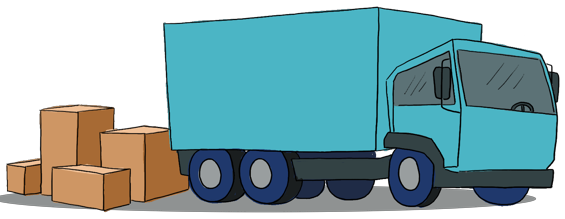
\includegraphics[width=0.85\linewidth]{Pi5_bai2}
		\vspace*{-10pt}
	\end{figure}
	\textit{Lời giải.} 	Ta sẽ dần dần chất các kiện hàng theo thứ tự tuỳ ý lên mỗi xe tải, theo dõi một cách cẩn thận và dừng lại vào ngay trước thời điểm khi xe bị ``quá tải". Khi đó, trên mỗi xe đều có nhiều hơn $2$ tấn hàng hoá. Vì vậy chỉ cần $5$ xe tải là đủ luôn chở được hết số hàng để trong các kiện hàng đó.
	\vskip 0.1cm
	Ta sẽ chỉ ra rằng  nếu chỉ cử đi $4$ xe chưa chắc đã đủ để chở đi được hết số kiện hàng. Ví dụ, có $13$ kiện hàng, mỗi kiện nặng đúng $\frac{10}{13}$ tấn. Khi đó mỗi xe chỉ chở được tối đa $3$ kiện hàng, vì $4$ kiện hàng bất kỳ có tổng trọng lượng là $\frac{40}{13} > 3$ (tấn). Vì thế với $4$ xe chỉ chở được tối đa $12$ kiện hàng.
	\vskip 0.1cm
	$\pmb{3.}$ Sau khi được sạc đầy pin, điện thoại di động của bạn An dùng đúng $6$ tiếng ở chế độ trò chuyện hoặc đúng $210$ tiếng ở chế độ chờ. Khi bạn An lên tàu hoả để đi du lịch, pin của bạn được sạc đầy $100\%$, và trên tàu không có ổ cắm sạc nên khi xuống ga, pin của bạn cũng vừa hết sạch. Biết rằng An đã nói chuyện với bạn bè đúng một nửa thời gian khi ngồi trên tàu, còn nửa thời gian còn lại đặt điện thoại ở chế độ chờ. Hỏi thời gian An đi trên tàu hoả là bao nhiêu lâu?
	\begin{figure}[H]
		\centering
		\vspace*{-5pt}
		\captionsetup{labelformat= empty, justification=centering}
		\includegraphics[width=0.85\linewidth]{Pi5_bai3}
		\vspace*{-5pt}
	\end{figure}
	\textit{Lời giải.} \textbf{\color{toancuabi}Cách} $\pmb{1}$: Một tiếng An nói chuyện và một tiếng An để chế độ chờ sử dụng hết $\frac{1}{6} + \frac{1}{210} = \frac{6}{35}$ dung lượng sạc đầy của pin. 
	\vskip 0.1cm
	Do thời gian An nói chuyện điện thoại và thời gian An để điện thoại ở chế độ chờ bằng nhau, nên An đã đi trên tàu với thời gian là
	\begin{align*}
		2\cdot \frac{35}{6} = \frac{35}{3} = 11\frac{2}{3} \text{ (giờ),}
	\end{align*}
	tức là $11$ tiếng $40$ phút.
	\vskip 0.1cm
	\textbf{\color{toancuabi}Cách} $\pmb{2}$: Nếu An trò chuyện trong $210 \times 6$ giờ và để chế độ chờ trong $210\times 6$  giờ thì pin điện thoại đã phải xả hết dung lượng những $210+6 = 216$ lần. Nhưng pin chỉ xả hết có đúng một lần, nên suy ra An chỉ trò chuyện trong $210\times 6 : 216 = \frac{35}{6}$ (giờ), và để điện thoại chờ trong từng đó thời gian. Vì vậy An đã ngồi $11\frac{2}{3}$ (giờ) trên tàu hoả.
	\vskip 0.1cm
	$\pmb{4.}$ Một nhóm học sinh đi bộ từ điểm hẹn tới bến xe buýt để kịp đón chuyến xe vào lúc $8$ giờ. Cũng vào thời điểm này, từ điểm tham quan, một chiếc xe buýt cũng xuất phát để tới kịp bến xe đón nhóm học sinh đó. Tuy  nhiên nhóm học sinh tới bến xe buýt khá sớm, vào lúc $6$ giờ $10$ phút, nên họ quyết định đi bộ tiếp tới điểm tham quan. Trên đường, các bạn đã gặp được xe buýt và lên xe đi tiếp.  Cuối cùng cả nhóm đến được điểm tham quan sớm hơn $20$ phút so với thời gian ấn định. Biết rằng vận tốc của xe buýt là $60$~km/h và vận tốc đi bộ của các em học sinh luôn không đổi. Hãy tìm vận tốc đi bộ của nhóm học sinh trước khi gặp xe buýt.
	\begin{figure}[H]
		\centering
		\vspace*{-5pt}
		\captionsetup{labelformat= empty, justification=centering}
		\includegraphics[width=0.9\linewidth]{Pi5_bai4}
		\vspace*{-10pt}
	\end{figure}
	\textit{Lời giải.} Ký hiệu $A$ là nhà ga, $B$ là điểm tham quan, $C$ là điểm trên đoạn thẳng $AB$ mà xe buýt gặp các bạn học sinh.
	\begin{figure}[H]
		\vspace*{-5pt}
		\centering
		\captionsetup{labelformat= empty, justification=centering}
		\begin{tikzpicture}[toancuabi]
			\draw (0,0) -- (6.5,0);
			\draw [fill=white] (0,0) circle (1.5pt) node [above] {$A$};
			\draw [fill=white] (2.5,0) circle (1.5pt) node [above] {$C$};
			\draw [fill=white] (6.5,0) circle (1.5pt) node [above] {$B$};
		\end{tikzpicture}
		\vspace*{-15pt}
	\end{figure}	
	Nhóm học sinh tiết kiệm được $20$ phút và xe buýt cũng vậy. Đồng thời, xe buýt tiết kiệm được $2$ lần quãng đường $AC$. Do đó xe buýt đi quãng đường $AC$ hết $10$ phút. Theo kế hoạch thời gian hẹn đón học sinh là $8$h, thực tế là xe gặp nhóm học sinh vào lúc $7h\,50$.
	\vskip 0.1cm
	Điều này suy ra rằng nhóm học sinh đã đi bộ từ $A$ tới $C$ mất thời gian là
	\begin{align*}
		7h\, 50 - 6h\, 10 = 100 \text{ (phút).}
	\end{align*}
	Thời gian đi quáng đường $AC$ của nhóm học sinh gấp thời gian đi của xe buýt số lần là
	\begin{align*}
		100 : 10 = 10 \text{ (lần).}
	\end{align*}
	Vậy vận tốc đi bộ của các em học sinh bằng $\frac{1}{10}$ vận tốc của xe buýt, tức là $6$ km/h.
	\vskip 0.1cm
	$\pmb{5.}$ 	Có $100$ chiếc xe ô tô đỗ liền nhau thành một hàng dọc bên lề đường, trong đó có $70$ chiếc xe hiệu Mercedes, còn lại là những xe nhãn hiệu khác. Trong các xe nhãn hiệu Mercedes có $30$ chiếc màu đỏ, $20$ chiếc màu vàng và $20$ chiếc màu hồng. Biết rằng không có hai xe Mercedes nào khác màu lại đỗ cạnh nhau. Em hãy chỉ ra rằng luôn tìm ra $3$ chiếc xe Mercedes cùng màu đỗ liên tiếp nhau.
	\begin{figure}[H]
		\centering
		\vspace*{-5pt}
		\captionsetup{labelformat= empty, justification=centering}
		\includegraphics[width=0.85\linewidth]{Pi5_bai5}
		\vspace*{-10pt}
	\end{figure}
	\textit{Lời giải.} Ta có $70$ chiếc Mercedes và $30$ xe nhãn hiệu ``khác". Theo điều kiện, mỗi xe Mercedes chỉ có thể đỗ cạnh một xe Mercedes có cùng màu với nó, hoặc cạnh một xe ``khác". Càng nhiều xe Mercedes cùng màu đỗ thành cặp cạnh nhau, càng cần ít các xe ``khác".
	\vskip 0.1cm
	Giả sử không có $3$ chiếc Mercedes cùng màu nào xếp cạnh nhau. Do tổng cộng số các cặp cùng màu của xe loại Mercedes là $35$, vậy phải có ít nhất $34$ xe ``khác" xếp ``xung quanh" chúng. Theo đề bài, chỉ có $30$ các xe ``khác". Đây là điều mâu thuẫn.
	\vskip 0.1cm
	Suy ra phải có $3$ chiếc xe Mercedes cùng màu đỗ cạnh nhau.
	\vskip 0.1cm
	$\pmb{6.}$ Một lớp học có $20$ em học sinh. Cô giáo chủ nhiệm của lớp tổ chức một số buổi tham quan vào mỗi ngày cuối tuần trong suốt năm học, mỗi buổi tham quan có ít nhất $4$ em học sinh tham gia. Em hãy chứng minh rằng có một buổi tham quan mà mỗi em học sinh tham gia buổi đó đều tham gia ít nhất $1/17$ tổng số tất cả các buổi tham quan của cả năm học.
	\begin{figure}[H]
		\centering
		\vspace*{-15pt}
		\captionsetup{labelformat= empty, justification=centering}
		\includegraphics[width=0.85\linewidth]{Pi5_bai6}
		\vspace*{-10pt}
	\end{figure}
	\textit{Lời giải.}	Gọi tổng số buổi tham quan là $n$, và cho mỗi em học sinh đều giữ lại vé cuả mỗi buổi thăm quan mà mình đã tham gia. Ta gọi một em học sinh là ``đáng thương"  nếu học sinh đó tham gia ít hơn $\frac{n}{17}$ buổi thăm quan. Chúng ta lấy bút đỏ đánh dấu tất cả các vé đã mua của tất cả các em học sinh ``đáng thương". 
	\vskip 0.1cm
	Giả sử trong mỗi buổi thăm quan đều có một vé bị đánh dấu đỏ. Khi đó có không ít hơn $n$ vé bị đánh dấu đỏ, và đóng góp vé của mỗi học sinh ``đáng thương" phải ít hơn $\frac{n}{17}$ vé. Suy ra số học sinh ``đáng thương" nhiều hơn $17$ em.
	\vskip 0.1cm
	Ta chọn ra đúng $17$ em  ``đáng thương".  Các em được chọn ra này có ít hơn $17\cdot \frac{n}{17}= n$  (vé), còn mỗi em trong số $3$ học sinh còn lại chỉ có tối đa $n$ vé, suy ra tổng số vé ít hơn $4n$. Mặt khác, trong mỗi buổi thăm quan đã bán ra ít nhất $4$ vé cho các em học sinh. Đây là điều mâu thuẫn.
	\vskip 0.1cm
	Vậy có ít nhất một buổi thăm quan mà không có vé nào bị đánh dấu đỏ, đó là điều phải chứng minh.
\end{multicols}
\newpage
\begingroup
\thispagestyle{toancuabinone}
\blfootnote{$^1$\color{toancuabi}Ottawa, Canada.}
\AddToShipoutPicture*{\put(60,733){\includegraphics[width=17.2cm]{../mathc.pdf}}}
%\AddToShipoutPicture*{\put(-2,733){\includegraphics[width=17.2cm]{../mathl.pdf}}} 
\AddToShipoutPicture*{\put(175,675){\includegraphics[scale=1]{../tieudea.pdf}}} 
\centering
\endgroup
\graphicspath{{../toancuabi/pic/}}
\vspace*{35pt}

\begin{multicols}{2}
	In this article, some problems of paths on boards are discussed.
	They highlight the relations of cells in same column or row.
	\vskip 0.2cm
	\PIbox{{\color{toancuabi}\textbf{\color{toancuabi}Example} (Who is the taller one?)}
	\vskip 0.1cm
	One hundred students are positioned in $10 \times 10$ grids,
	each of the rows and columns contains exactly $10$ students.
	From each of the $10$ columns the \textit{shortest} student is selected,
	and the \textit{tallest} of these $10$ students is tagged as $T$.
	Next the \textit{tallest} student from each rows is selected,
	and from these $10$ students the \textit{shortest} is tagged as $S$.
	Which of the two tagged students is the taller if they are two different people?}
	\vskip 0.2cm
	\textit{Solution.}
	If $S$ and $T$ are in the same column, then $T$ is among the shortests of each column,
	so $T$ is the shortest in its own column, thus $T$ is shorter than $S$.
	If $S$ and $T$ are in the same row, then $S$ is among the tallests of each column,
	so it is the tallest in its own row, thus $T$ is shorter than $S$.
	\begin{figure}[H]
	\vspace*{-5pt}
	\centering
	\captionsetup{labelformat= empty, justification=centering}
	\begin{tikzpicture}[scale=0.9, toancuabi]
		\draw (0,0) grid (5,5);
		\draw (1.5,1.5) node{$\color{red}S$};
		\draw (3.5,1.5) node{$I$};
		\draw (3.5,3.5) node{$\color{cackithi!40}T$};
	\end{tikzpicture}
	\vspace*{-5pt}
	\end{figure}
	If $S$ and $T$ are in different rows and colums,
	then there exists $I$ at the intersection of the row of $S$ and the column of $T$.
	By definition, $T$ is shorter than $I$ and $I$ is shorter than $S$,
	thus $T$ is shorter than $S$.
	\vskip 0.1cm
	Therefore, ${S}$ is the taller one.
	\vskip 0.2cm
	\PIbox{{\color{toancuabi}\textbf{\color{toancuabi}Example} (How many ways to form the name?)}
	\vskip 0.1cm
	Thanh filled a triangle of squares with the letters of her name, as shown below.
	She counted all the $5-$letter paths that form her name T--H--A--N--H,
	each starts from the T letter in the middle of the bottom row,
	then goes left, right, or up. An example is also shown in the diagram.
	What number did she get?}
	\vskip 0.2cm
	\begin{figure}[H]
		\vspace*{-5pt}
		\centering
		\captionsetup{labelformat= empty, justification=centering}
		\renewcommand{\arraystretch}{1.2}
		\begin{tabular}{ccccccccc}
		&   &   &   & H                                                &                                                  &                                                  &   &   \\
		&   &   & H & N                                                & H                                                &                                                  &   &   \\
		&   & H & N & A                                                & \cellcolor{cackithi!40}N & \cellcolor{cackithi!40}H &   &   \\
		& H & N & A & \cellcolor{cackithi!40}H& \cellcolor{cackithi!40}  A  & N                                                & H &   \\
		H & N & A & H & \cellcolor{cackithi!40}T & H                                                & A                                                & N &  H 
	\end{tabular} 
	\vspace*{-10pt}
	\end{figure}
	\textit{Solution.}
	Consider the \textit{``half"} triangle shown in the diagram below.
	It is easy to see that in each path, there is two choices at each steps.
	One example is shown in the figure, when two As can be chosen after a $H$.
	\begin{figure}[H]
	\vspace*{-5pt}
	\centering
	\captionsetup{labelformat= empty, justification=centering}
	\renewcommand{\arraystretch}{1.2}
	\begin{tabular}{ccccl}
		&   &                                                  &                                                  &  H                                                 \\
		&   &                                                  &  H                                                 &  N                                                 \\
		&   &  H                                                 &  N                                                 &  A                                                 \\
		&  H  &  N                                                 & \cellcolor{duongvaotoanhoc!40}  A &  H                                                 \\
		H  &  N  & \cellcolor{duongvaotoanhoc!40}  A  & \cellcolor{cackithi!40}  H  & \cellcolor{cackithi!40}  T 
	\end{tabular}
	\vspace*{-10pt}
	\end{figure}
	Therefore there are $2^4=16$ paths for a half triangle.
	In total there are $2\cdot 16-1=31$,
	because the vertical path formed by all the squares in the $T$ column
	is shared by both half triangles.
	\vskip 0.1cm
	Thus, the number that Thanh got is $31.$
	\vskip 0.1cm
	\PIbox{{\color{toancuabi}\textbf{\color{toancuabi}Example} (What would be the largest number?)}
	\vskip 0.1cm
	In each square of the $n \times n$, $n \ge 4$ chessboard,
	Antoine writes a number according to the following rules:
	\vskip 0.1cm
	$i.$ The number in each square is one of $1,2,\ldots,n^2$.
	\vskip 0.1cm
	$ii.$ The two numbers, in two neighbouring squares that share the same side, differ less than $3$.
	\vskip 0.1cm
	$iii.$ The number $3$ is written in one of the square.
	\vskip 0.1cm
	What is the largest number could Antoine writes on the board?}
	\vskip 0.2cm
	\textit{Solution.}
	Let $m$ be the maximal number that can be written on the board.
	\begin{figure}[H]
	\vspace*{-5pt}
	\centering
	\captionsetup{labelformat= empty, justification=centering}
	\begin{tikzpicture}[toancuabi]
			\filldraw[cackithi!40] (0,3) rectangle (5,4);
			\filldraw[cackithi!40] (3,0) rectangle (4,5);
			\draw (0,0) grid (5,5);
			\draw (1.5,3.5) node {$3$};
			\draw (3.5,1.5) node {$m$};
			\draw (3.5,3.5) node {$i$};
	\end{tikzpicture}
	\vspace*{-10pt}
	\end{figure}
	In the figure above, there are atmost $n-1$ squares on the row of $3$,
	not including the square containing $3$, 
	from the number $3$ to the intersection $i$ with the column of $m$,
	Similarly there are atmost $n-1$ squares on the column of $m$,
	not including the square containing $m$, 
	from the intersection $i$ with the column of $m$ to the number $m$.
	Thus the difference between $m$ and $3$ can not be more than
	$2\cdot (n-1)+ 2\cdot (n-1)=4(n-1)$.
	\vskip 0.1cm
	Therefore, the largest value of $m$ can be $3+4(n-1)={4n-1.}$
	\vskip 0.2cm
	\PIbox{{\color{toancuabi}\textbf{\color{toancuabi}Example} (Colouring the paths)}
	\vskip 0.1cm
	In the $4 \times 4$ grid below each cell at row $i$ and column $j$ contains the value equal to $i \times j.$
	A \textit{path} in the grid is a sequence of squares,
	such that consecutive squares share an edge and no square occurs twice in the sequence.
	Furthermore, the \textit{score} of a path is the sum of the point values of all squares in the path.
	\vskip 0.1cm
	Determine the highest possible score of a path that begins with the bottom left corner of the grid 
	(where the number $1$ stands) and ends with the top right corner (where the number $16$ stands.)}
	\vskip 0.2cm
	\begin{figure}[H]
	\vspace*{-5pt}
	\centering
	\captionsetup{labelformat= empty, justification=centering}
	\begin{tikzpicture}[toancuabi]
		\draw (0,0) grid (4,4);
		\draw (0.5 , 0.5) node {$1$};
		\draw (0.5 , 1.5) node {$2$};
		\draw (0.5 , 2.5) node {$3$};
		\draw (0.5 , 3.5) node {$4$};
		\draw (1.5 , 0.5) node {$2$};
		\draw (1.5 , 1.5) node {$4$};
		\draw (1.5 , 2.5) node {$6$};
		\draw (1.5 , 3.5) node {$8$};
		\draw (2.5 , 0.5) node {$3$};
		\draw (2.5 , 1.5) node {$6$};
		\draw (2.5 , 2.5) node {$9$};
		\draw (2.5 , 3.5) node {$12$};
		\draw (3.5 , 0.5) node {$4$};
		\draw (3.5 , 1.5) node {$8$};
		\draw (3.5 , 2.5) node {$12$};
		\draw (3.5 , 3.5) node {$16$};
	\end{tikzpicture}
	\vspace*{-10pt}
	\end{figure}
	\textit{Solution.}
	Let us colour the squares of the grid with a chessboard pattern of black and white,
	starting with black in the bottom left--hand corner, as show below on the left diagram.
	A path in the grid will alternate between black and white squares,
	beginning and ending on black.
	Thus, any path cannot contain all $8$ white squares.
	\vskip 0.1cm
	\begin{figure}[H]
		\vspace*{-5pt}
		\centering
		\captionsetup{labelformat= empty, justification=centering}
		\begin{tikzpicture}[toancuabi]
			\foreach \y in {0,2}{
			\foreach \x in {0,2}{
					\fill[cackithi!40] (\x,\y) rectangle (1+\x,1+\y) rectangle (2+\x,2+\y);}}
			\draw (0,0) grid (4,4);
			\draw (0.5 , 0.5) node {$1$};
			\draw (0.5 , 1.5) node {$2$};
			\draw (0.5 , 2.5) node {$3$};
			\draw (0.5 , 3.5) node {$4$};
			\draw (1.5 , 0.5) node {$2$};
			\draw (1.5 , 1.5) node {$4$};
			\draw (1.5 , 2.5) node {$6$};
			\draw (1.5 , 3.5) node {$8$};
			\draw (2.5 , 0.5) node {$3$};
			\draw (2.5 , 1.5) node {$6$};
			\draw (2.5 , 2.5) node {$9$};
			\draw (2.5 , 3.5) node {$12$};
			\draw (3.5 , 0.5) node {$4$};
			\draw (3.5 , 1.5) node {$8$};
			\draw (3.5 , 2.5) node {$12$};
			\draw (3.5 , 3.5) node {$16$};
		\end{tikzpicture}
		\caption{\small\textit{\color{toancuabi}Figure $1$. Alternate colouring.}}
		\vspace*{-10pt}
	\end{figure}
	\begin{figure}[H]
	\vspace*{-5pt}
	\centering
	\captionsetup{labelformat= empty, justification=centering}
	\begin{tikzpicture}[toancuabi]
		\draw (0,0) rectangle (4,4);
		\draw (1,0) grid (2,1);
		\draw (0,2) -- (4,2) -- (4,1);
		\draw (1,3) -- (4,3);
		\draw (0.5 , 0.5) node {$1$};
		\draw (0.5 , 1.5) node {$2$};
		\draw (0.5 , 2.5) node {$3$};
		\draw (0.5 , 3.5) node {$4$};
		\draw (1.5 , 0.5) node {$2$};
		\draw (1.5 , 1.5) node {$4$};
		\draw (1.5 , 2.5) node {$6$};
		\draw (1.5 , 3.5) node {$8$};
		\draw (2.5 , 0.5) node {$3$};
		\draw (2.5 , 1.5) node {$6$};
		\draw (2.5 , 2.5) node {$9$};
		\draw (2.5 , 3.5) node {$12$};
		\draw (3.5 , 0.5) node {$4$};
		\draw (3.5 , 1.5) node {$8$};
		\draw (3.5 , 2.5) node {$12$};
		\draw (3.5 , 3.5) node {$16$};
	\end{tikzpicture}
	\caption{\small\textit{\color{toancuabi}Figure $2$. Path with maximal value.}}
	\vspace*{-10pt}
	\end{figure}
	The path from $1$ to $16$ with highest possible score should contains all squares
	except for the square containing $2$ at the bottom row, as show above in the right diagram.
	The sum of the values for all the squares in this path is 
	\begin{align*}
		&(1\!+\!2\!+\!3\!+\!4)\!+\!(2\!+\!4\!+\!6\!+\!8)\\
		&\!+\!(3\!+\!6\!+\!9\!+\!12)\!+\!(4\!+\!8\!+\!12\!+\!16) \\
		= \,&(1\!+\!2\!+\!3\!+\!4)(1\!+\!2\!+\!3\!+\!4) \!=\! 10^2 \!=\! 100,
	\end{align*}		
	Thus, the score of the path is $100-2={98}.$
\end{multicols}